\section{Auswertung}
\label{sec:auswertung}

Im Folgenden wird die gemessene Magnetfeldstärke für verschiedene
Tiefen der Hall-Sonde in den Elektromagneten visualisiert, sowie die
effektive Masse von Elektronen in GaAs bestimmt.
Die Auswertung ist mit Hilfe der \textit{python}-Pakete
\textit{scipy\_curvefit} und \textit{numpy} bewerkstelligt worden.

\subsection{Magnetfeld}

Die gemessenen Werte des $B$-Feldes sind in Abbildung~\ref{fig:B} dargestellt.
Auf eine Ausgleichrechnung für die Ermittlung von $B\ua{max}$ wird verzichtet,
da in dem Bereich um den Hochpunkt von $B(s)$ ausreichend viele Messpunkte vorliegen.

\begin{figure}
  \centering
  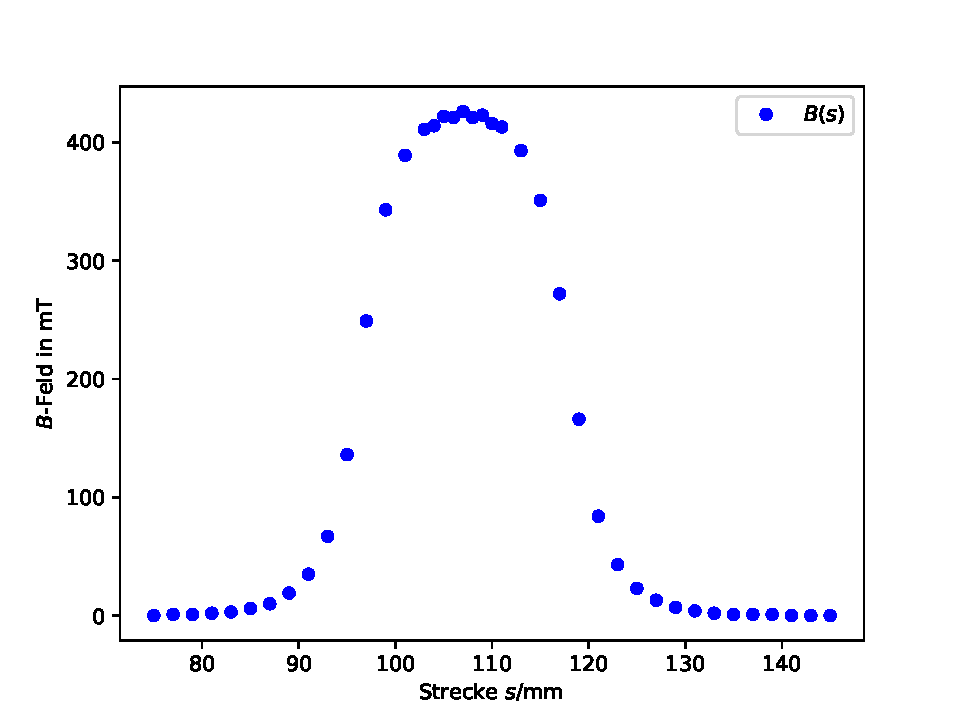
\includegraphics[width = 0.9\textwidth]{Plots/B.pdf}
  \caption{Gemessene Werte des Magnetfeldes $B$ für verschiedene Tiefen der Hall-Sonde.}
  \label{fig:B}
\end{figure}

\begin{figure}
  \centering
  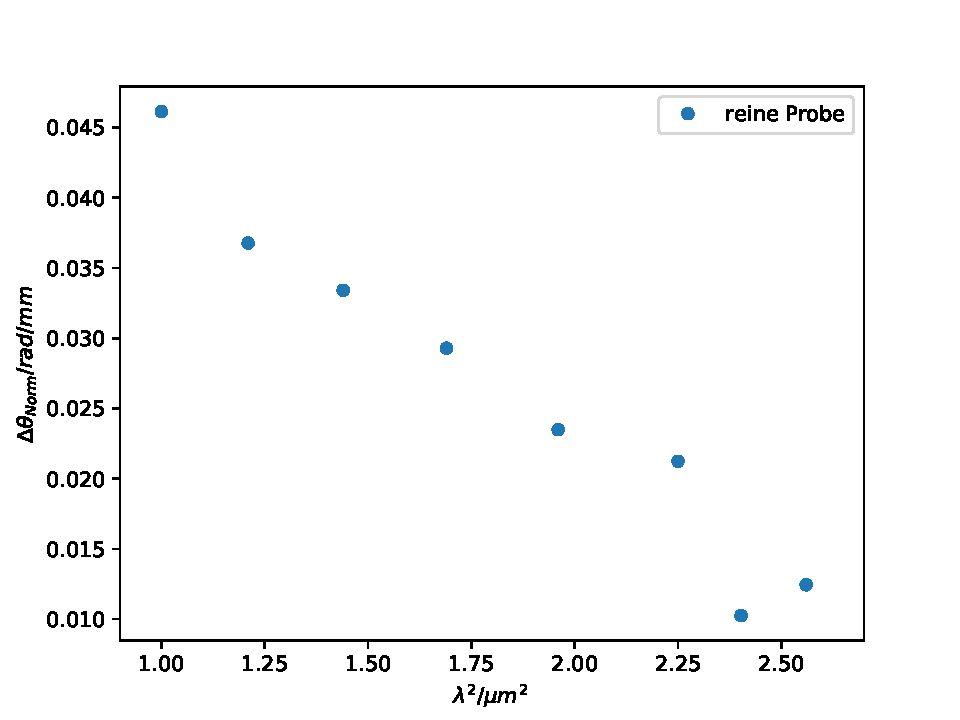
\includegraphics[width = 0.9\textwidth]{Plots/hr_GaAs.pdf}
  \caption{Normierte Faraday-Rotationswinkel der reinen GaAs Probe für verschiedene Wellenlängen $\lambda$.}
  \label{fig:hr}
\end{figure}

\begin{table}
\centering
\caption{Messwerte der reinen GaAs Probe, mit der Dicke $d = \SI{5.11}{\milli\meter}$. $\theta$ beschreibt den Faraday-Rotationswinkel
und $\theta_{\symup{Norm}}$ den über die Dicke normierten Faraday-Rotationswinkel.
$B_+$ und $B_-$ indizieren die Polung des Magnetfeldes.}
\label{tab:hr}
\begin{tabular}{S S S S S }
\toprule
{$\lambda / \si{\micro\meter}$} & {$\theta(B_+) / \si{\radian}$} & {$\theta(B_-) / \si{\radian}$}  & {$\theta / \si{\radian}$} & {$\theta\ua{Norm} / \si{\radian\per\mm}$}   \\
\midrule
1.00  & 2.40  & 2.87  & 0.236  & 0.046\\
1.10  & 2.43  & 2.80  & 0.188  & 0.037\\
1.20  & 2.45  & 2.79  & 0.171  & 0.033\\
1.30  & 2.48  & 2.78  & 0.150  & 0.029\\
1.40  & 2.53  & 2.77  & 0.120  & 0.023\\
1.50  & 2.51  & 2.73  & 0.109  & 0.021\\
1.55  & 2.73  & 2.83  & 0.052  & 0.010\\
1.60  & 2.71  & 2.83  & 0.064  & 0.012\\
\bottomrule
\end{tabular}
\end{table}


\begin{figure}
  \centering
  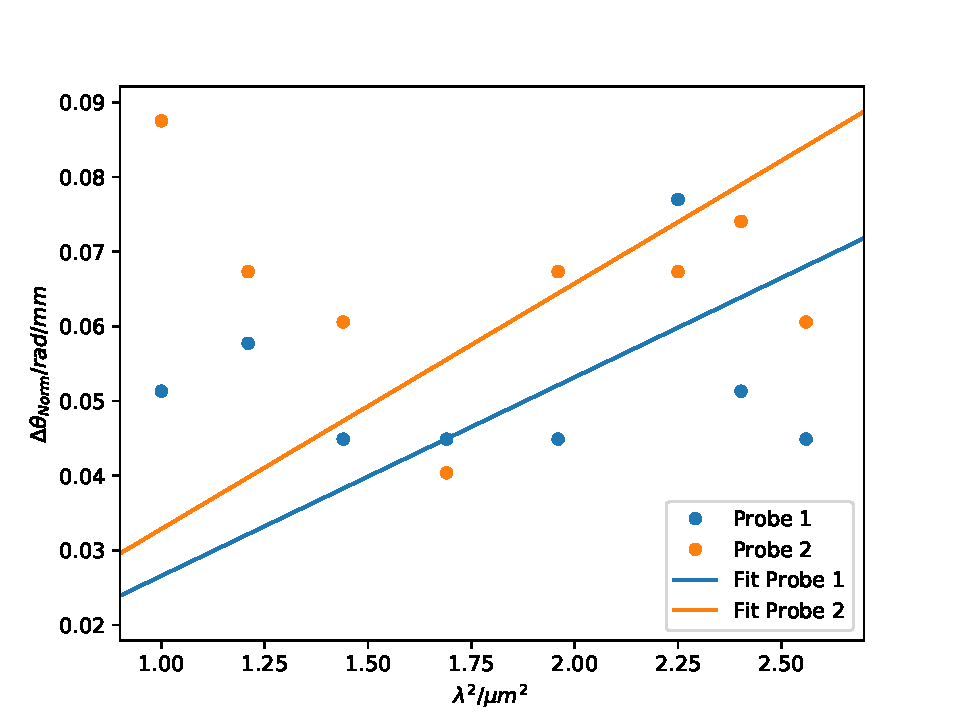
\includegraphics[width = 0.9\textwidth]{Plots/dotiert_GaAs.pdf}
  \caption{Differenz der normierten Faraday-Rotationswinkel der dotierten GaAs Probe und der reinen GaAs Probe für verschiedene Wellenlängen $\lambda$.}
  \label{fig:dot}
\end{figure}

\begin{table}
\centering
\caption{Messwerte der dotierten GaAs Probe, mit der Dicke $d = \SI{1.36}{\mm}$. $\theta_1$ beschreibt den Faraday-Rotationswinkel und $\Delta\theta_{\symup{1, Norm}}$ den mit der Dicke $d$ normierten Wert abzüglich des normierten Faraday-Rotationswinkels der hochreinen Probe.}
\label{tab:probe1}
\begin{tabular}{S S S S S S}
\toprule
{$\lambda / \si{\micro\meter}$} & {$\theta_1(B_+) / \si{\radian}$} & {$\theta_1(B_-) / \si{\radian}$} & {$\theta_1 / \si{\radian}$} & $\theta_{\symup{1, Norm}} / \si{\radian\per\mm}$ & {$\Delta\theta_{\symup{1, Norm}} / \si{\radian\per\m}$}  \\
\midrule
1.00  & 2.52  & 2.57  & 0.070  & 0.051  & 0.005\\
1.10  & 2.51  & 2.56  & 0.079  & 0.058  & 0.021\\
1.20  & 2.56  & 2.57  & 0.061  & 0.045  & 0.012\\
1.30  & 2.55  & 2.59  & 0.061  & 0.045  & 0.016\\
1.40  & 2.57  & 2.56  & 0.061  & 0.045  & 0.021\\
1.50  & 2.58  & 2.55  & 0.105  & 0.077  & 0.056\\
1.55  & 2.70  & 2.68  & 0.070  & 0.051  & 0.041\\
1.60  & 2.70  & 2.68  & 0.061  & 0.045  & 0.032\\
\bottomrule
\end{tabular}
\end{table}

\begin{table}
\centering
\caption{Messwerte der dotierten GaAs Probe, mit der Dicke $d = \SI{1.296}{\mm}$. $\theta_2$ beschreibt den Faraday-Rotationswinkel und $\Delta\theta{_\symup{1, Norm}}$ den mit der Dicke $d$ normierten Wert abzüglich des normierten Faraday-Rotationswinkels der hochreinen Probe.}
\label{tab:probe2}
\begin{tabular}{S S S S S S }
\toprule
{$\lambda / \si{\micro\meter}$} & {$\theta_2(B_+) / \si{\radian}$} & {$\theta_2(B_-) / \si{\radian}$} & {$\theta_2 / \si{\radian}$} & $\theta_{\symup{2, Norm}} / \si{\radian\per\mm}$ & {$\Delta\theta{_\symup{2, Norm}} / \si{\radian\per\milli\meter}$}  \\
\midrule
1.00  & 2.66  & 2.79  & 0.113  & 0.088  & 0.041\\
1.10  & 2.67  & 2.74  & 0.087  & 0.067  & 0.031\\
1.20  & 2.68  & 2.72  & 0.079  & 0.061  & 0.027\\
1.30  & 2.67  & 2.69  & 0.052  & 0.040  & 0.011\\
1.40  & 2.69  & 2.74  & 0.087  & 0.067  & 0.044\\
1.50  & 2.79  & 2.73  & 0.087  & 0.067  & 0.046\\
1.55  & 2.83  & 2.87  & 0.096  & 0.074  & 0.064\\
1.60  & 2.82  & 2.84  & 0.079  & 0.061  & 0.048\\
\bottomrule
\end{tabular}
\end{table}


\begin{equation}
  \label{eqn:eff_m_1}
  m^*_1 = \SI{6.3e-32(15)}
\end{equation}

\begin{equation}
  \label{eqn:eff_m_2}
  m^*_2 = \SI{7.2e-32(20)}
\end{equation}
